\chapter{DOE - Teilfaktorielle Versuchspläne}
\label{sec: Hauptkapitel 1}

\section{Aufgabenstellung}
    In dieser Laboraufgabe wurde die Frequenzlage eines Modes in Abhängigkeit von vier 
    zusätzlichen Massen untersucht. Die Eigenmoden des Flugzeugs ohne zusätzliche Massen 
    wurden bereits in Kapitel 2 bestimmt. Der Fokus dieses Versuchs liegt speziell auf dem 
    ersten Mode, dessen Frequenz ohne Massen 5,048 Hz beträgt.  
    \\

    \noindent
    Die Untersuchung erfolgte gemäß der Aufgabenstellung anhand eines teilfaktoriellen 
    Versuchsplans. Dabei wurden verschiedene Kombinationen der Massen betrachtet, wobei 
    ausschließlich die Haupteffekte von Interesse sind.

%================================================================================

\section{Versuchsaufbau}
    Für den Versuch wurde ein teilfaktorieller Versuchsplan mit vier Faktoren (Massen) 
    und zwei Stufen (-1 und +1) angewendet. Ziel war es, den Einfluss der zusätzlichen Massen 
    auf die Frequenzlage des ersten Modes des Tragflügels zu bestimmen.  
    \\

    \noindent
    Da jeder Faktor zwei Stufen besitzt, würde ein vollständiger vollfaktorieller Versuchsplan 
    insgesamt \(2^4 = 16\) Kombinationen erfordern. Da in der Aufgabenstellung explizit ein 
    teilfaktorieller Versuchsplan vorgegeben wurde, wurde die Anzahl der Versuche auf 
    8 Kombinationen reduziert. Es handelt sich um einen Versuchsplan der Auflösung IV, 
    bei dem die Haupteffekte eindeutig von den Zweifachwechselwirkungen getrennt werden können. 
    Allerdings lassen sich Zweifachwechselwirkungen nicht mehr von Dreifachwechselwirkungen unterscheiden.
    \\

    \noindent
    Der Beschleunigungssensor blieb während des gesamten Versuchs an einer festen Position 
    (Position 5, rot). Die genaue Anordnung der Sensor- und Massenpositionen ist in 
    Abbildung \ref{fig: Flieger_diskretisiert} dargestellt.

    % Bild - Diskretisiertes Modellflugzeug
    %--------------------------------------
    \begin{figure}[H]
        \centering
        \includegraphics[width=0.95\textwidth]{Flieger_diskretisiert_Comp.png}
        \caption{Diskretisiertes Modellflugzeug mit Sensor- und Massenpositionen}
        \label{fig: Flieger_diskretisiert}
    \end{figure}

    \noindent
    Je nach getesteter Kombination wurden die vier Massen an den vordefinierten Positionen 
    des Tragflügels angebracht. Die Platzierung der Massen erfolgte nach folgendem Schema:

    \begin{itemize}
        \item Masse 1: Position 1 (rot), 41 g  
        \item Masse 2: Position 5 (rot), 44 g  
        \item Masse 3: Position 1 (blau), 42 g  
        \item Masse 4: Position 5 (blau), 44 g  
    \end{itemize}

    \noindent
    Für jede Kombination wurden drei Messungen durchgeführt. Aus diesen Messungen wurden 
    anschließend der Mittelwert der Frequenz, die Standardabweichung sowie die Varianz berechnet.
%================================================================================
\section{Ergebnisse}
    Nach der Durchführung der Messungen wurden die Frequenzlage für jede getestete 
    Kombination analysiert. Für jede Konfiguration wurden dabei drei Messungen durchgeführt, 
    um die Frequenzlage möglichst präzise zu bestimmen. Anschließend wurden der Mittelwert der 
    Frequenz, die Standardabweichung und die Varianz berechnet.  
    \\

    \noindent
    Die Messergebnisse sind in Abbildung \ref{fig: Aufgabe4_Messungen} dargestellt.
    
    % Bild - Messergebnisse
    \begin{figure}[H]
        \centering
        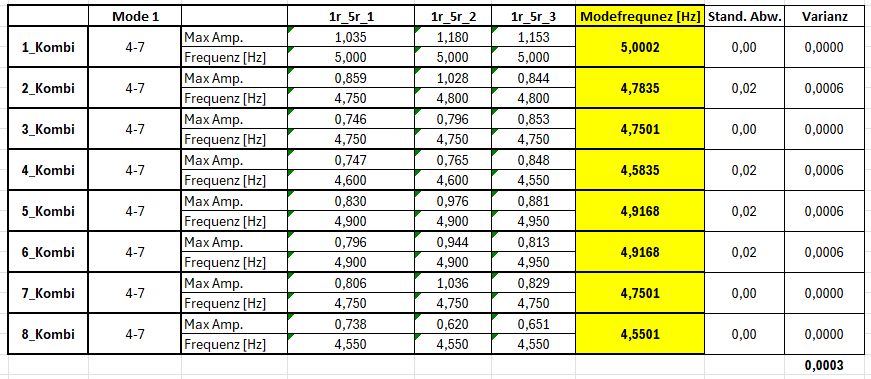
\includegraphics[width=0.95\textwidth]{Aufgabe4_Messungen.png}
        \caption{Bestimmung der Modefrequenz aus drei Messungen}
        \label{fig: Aufgabe4_Messungen}
    \end{figure}
    
    \noindent
    Basierend auf den ermittelten Frequenzwerten wurde ein teilfaktorieller Versuchsplan erstellt. 
    Dieser zeigt die berechneten Haupteffekte sowie Wechselwirkungen zwischen den Massen.  
    Die Ergebnisse des Versuchsplans sind in Abbildung \ref{fig: Teilfaktorieller_Versuchsplan} dargestellt.
    
    % Bild - Teilfaktorieller Versuchsplan
    \begin{figure}[H]
        \centering
        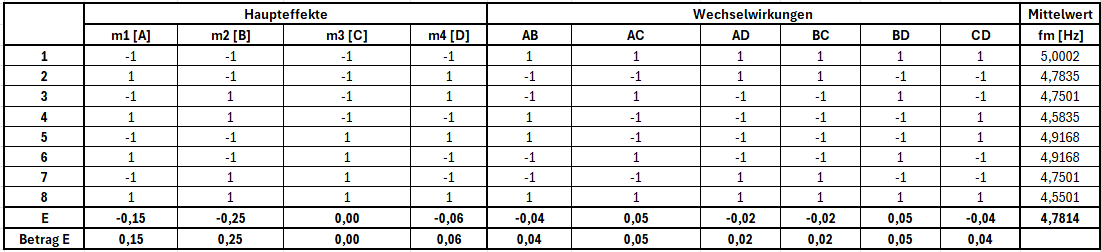
\includegraphics[width=0.95\textwidth]{Teilfaktorieller_Versuchsplan.png}
        \caption{Teilfaktorieller Versuchsplan mit berechneten Haupteffekten}
        \label{fig: Teilfaktorieller_Versuchsplan}
    \end{figure}
    
    \noindent
    Um die Signifikanz der einzelnen Effekte zu bestimmen, wurde die vorher berechnete Varianz mit 
    der Quantilfunktion verrechnet. Daraus wurde das Signifikanzniveau ermittelt, welches die signifikanten 
    und nicht signifikanten Effekte im Vergleich zeigt. Die grafische Darstellung der Signifikanzanalyse 
    ist in Abbildung \ref{fig: Signifikanzniveau} zu sehen.
    
    % Bild - Signifikanzniveau
    \begin{figure}[H]
        \centering
        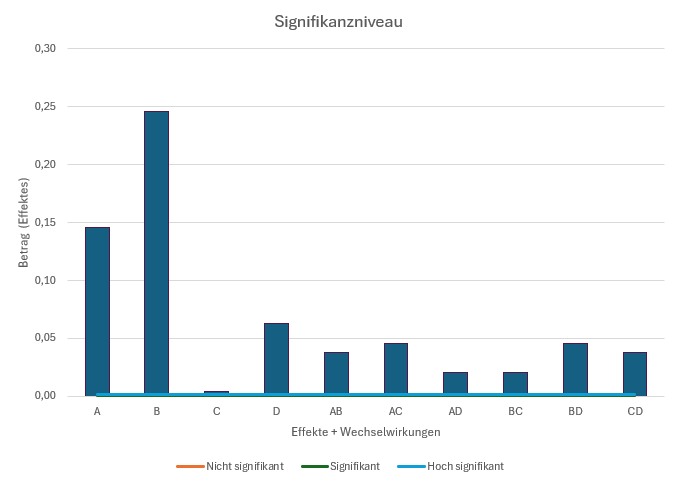
\includegraphics[width=0.95\textwidth]{Signifikanzniveau.png}
        \caption{Signifikanzanalyse der Haupteffekte und Wechselwirkungen}
        \label{fig: Signifikanzniveau}
    \end{figure}

    \noindent
    Die Signifikanzanalyse zeigt, dass alle Haupteffekte und Wechselwirkungen hoch signifikant sind, 
    mit Ausnahme des Faktors C, welcher der Masse 3 entspricht. Diese Masse war hinten an der Finne des Flugzeugs angebracht. 
    Es ist auffällig, dass Masse 3 keinen Einfluss zeigt, während Masse 4 (Faktor D) hoch signifikant ist.  
    Da beide Massen annähernd gleich schwer sind und das Flugzeug weitgehend symmetrisch aufgebaut ist, 
    wäre zu erwarten, dass entweder beide Massen (Masse 3 und 4) einen Einfluss haben oder beide keinen.  